\documentclass[14pt, a4paper]{article}

\usepackage[T2A]{fontenc}
\usepackage[utf8]{inputenc}
\usepackage[english, russian]{babel}

\usepackage{amsmath}
\usepackage{float}
\usepackage{graphicx}
\graphicspath{{./images/}}

\begin{document}
    \thispagestyle{empty}

    \begin{center}
        Министерство науки и высшего образования Российской Федерации

        Федеральное государственно автономное образовательное учреждение высшего образования

        <<Омский государственный технический университет>>

        \vspace{1cm}
        Факультет информационных технологий и компьютерных систем

        Кафедра <<Прикладная математика и фундаметральная информатика>>

        \vspace{3cm}
        \textbf{Лабораторная работа}

        по дисциплине <<Операционные системы>>
    \end{center}
    
    \vspace{3cm}
    \begin{flushright}    
        \begin{tabular}{ r r }
            Студента & Курпенова Куата Ибраимовича \\
            \cline{2-2}
            & \tiny{фамилия, имя, отчество полностью} \\

            Курс & 2, группа ФИТ-212 \\
            \cline{2-2}
            Направление & 02.03.02 Прикладная математика \\
            \cline{2-2}
            & и фундаментальная информатика \\
            \cline{2-2}
            & \tiny{код, наименование} \\

            Руководитель & ассистент \\
            \cline{2-2}
            & \tiny{должность, ученая степень, звание} \\
            & Грицай А. С. \\
            \cline{2-2}
            & \tiny{фамилия, инициалы} \\

            Выполнил & \\
            \cline{2-2}
            & \tiny{дата, подпись студента(ки)} \\
        \end{tabular}
    \end{flushright}
    
    \vspace*{\fill}
    \begin{center}
        Омск 2022
    \end{center}

    \newpage

    \section*{Задание 1}

    Разработать в Linux программу, которая получает хэндлы стандартного ввода и вывода, выводит числовые с комментариями значения этих хэндлов, затем, используя стандартный ввод системными функциями небуферизованного ввода-вывода ReadFile или WriteFile, делает приглашение для ввода, вводит любой текст и выводит его с предуведомлением, что он предварительно введен в программу, обеспечивая в этой системе вывод приглашения на ввод данных со стандартного ввода только в случае использовании ввода с консоли, при переадресации этого ввода на входной файл приглашение отображаться не должно. При переадресации стандартного вывода в файл отображение приглашения в случае ввода с консоли должно принудительно появляться на экране, а не в файле, на который переадресуется вывод. Числовые значения хэндлов стандартных ввода и вывода в этом варианте выводить не нужно.

    \subsection*{Решение}

    \begin{figure}[H]
        \centering
        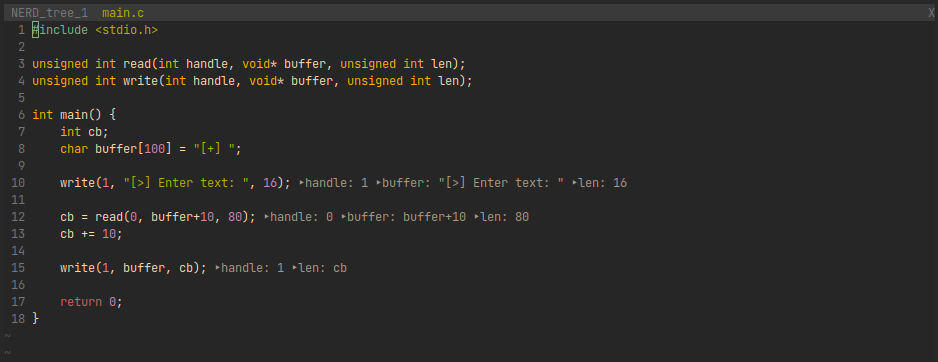
\includegraphics[width=\textwidth]{images/lab1/solution.png}
        \caption{Код программы main.c}
    \end{figure}

    \begin{figure}[H]
        \centering
        \includegraphics[width=\textwidth]{images/lab1/result.png}
        \caption{Вывод программы main.c}
    \end{figure}

    \newpage

    \section*{Задание 2}

    Результат выполнения лабораторной работы должен состоять из двух программ для Linux. Первая программа должна создавать текстовый файл, вводя данные со стандартного ввода. (Более детально: открывает файл для записи, читает текст со стандартного ввода и выводит этот прочитанный текст в файл.) Вторая программа открывает тот же файл (созданный перед этим другой программой) для чтения и хэндл, полученный при этом открытии, запоминает в 1-й переменной для хэндла. Используя этот хэндл, далее с помощью функции dup() получается новое значение хэндла для доступа к тому же файлу (2-й хэндл). Еще раз открывается тот же файл, запоминая 3-е значение хэндла. С помощью первого хэндла программа позиционирует чтение для 10-й позиции файла от начала этого файла. Далее программа должна выводить числовые значения всех трех хэндлов на экран. Используя по очереди все 3 хэндла, из файла читаются по 7 символов и тут же эти три прочитанных текста выводятся на экран, каждая в своей строке. Результаты вывода объяснить.

    \subsection*{Решение}

    \begin{figure}[H]
        \centering
        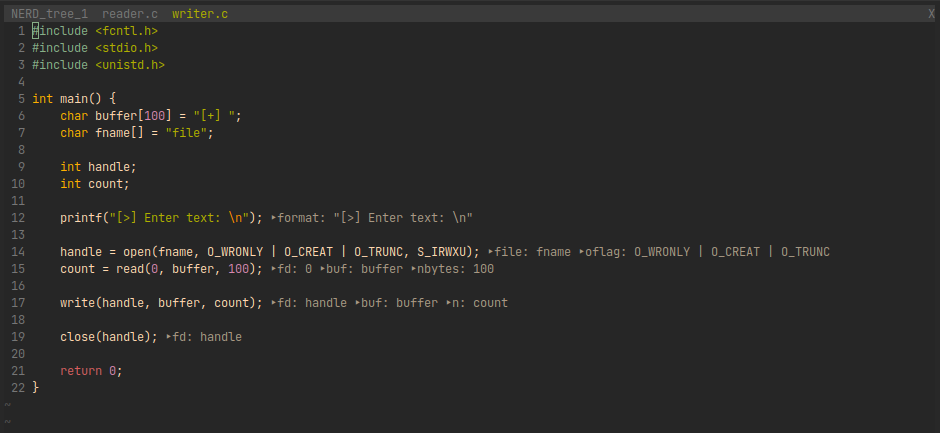
\includegraphics[width=\textwidth]{images/lab2/writer.png}
        \caption{Код программы writer.c}
    \end{figure}

    \begin{figure}[H]
        \centering
        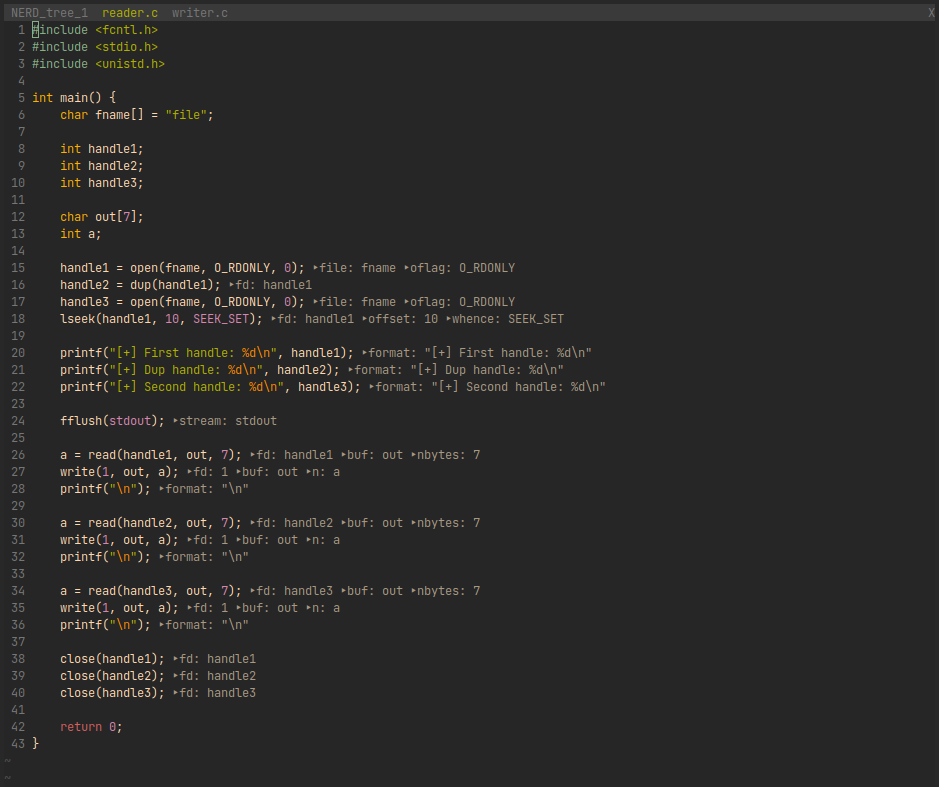
\includegraphics[width=\textwidth]{images/lab2/reader.png}
        \caption{Код программы reader.c}
    \end{figure}

    \begin{figure}[H]
        \centering
        \includegraphics[width=\textwidth]{images/lab2/result.png}
        \caption{Результат работы программ writer.c и reader.c}
    \end{figure}

    \newpage

    \section*{Задание 3}

    Разработать программу для Windows, которая должна запускаться в двух экземплярах - каждый в своем окне командной оболочки FAR или из ПРОВОДНИКа операционной системы. Программа использует заранее подготовленный текстовый файл. Она пытается открыть этот файл для чтения с указываемым при этом запрете для других использовать этот файл. По результатам выполнения системной функции открытия на экран выдается сообщение - удалось ли открыть файл и, если не удалось по причине отсутствия доступа к одновременно выполняемым программам, то сообщение именно об этой причине. При отсутствии указанного в программе файла после сообщения об этом отсутствии программа прекращает работу. При его наличии, но невозможности продолжения действий из-за блокировки, установленной другим экземпляром запущенной программы, выполняется ожидание освобождения файла от блокировки. При отсутствии указанной причины доступа программа должна ждать освобождения файла. В обоих случаях - ожидания освобождения или исходной доступности - программа читает из этого файла все находящиеся в нем данные и выводит их на экран. Сообщения должны выводиться цветные и в середине консольного окна.

    \begin{figure}[H]
        \centering
        \includegraphics[width=\textwidth]{images/lab3/main.png}
        \caption{Код программы main.c}
    \end{figure}

    \begin{figure}[H]
        \centering
        \includegraphics[width=\textwidth]{images/lab3/result.png}
        \caption{Результат работы программ main.c}
    \end{figure}

    \newpage

    \section*{Задание 4}

    Разработать программу для Linux, которая должна запускаться в двух экземплярах, каждый со своей виртуальной консоли. Программа использует заранее подготовленный текстовый файл. Она открывает этот файл, при невозможности этого действия выдается сообщение и прекращает выполнение. После успешного открытия файла делается попытка установить на весь файл многопользовательскую блокировку по записи. По результатам попытки выполнения блокировки – на экран выдается сообщение о его реализации или текущей невозможности это сделать. При невозможности установить блокировку сразу, программа задает блокировку с ожиданием ее выполнения. По установлении блокировки доступа программа читает из этого файла все находящиеся в нем данные и выводит их на экран. Затем программа делает задержку выполнения («засыпает») на 7 или 8 секунд, после чего снимает блокировку. Сообщения должны выводиться цветные и в середине экрана.

    \subsection*{Решение}

    \begin{figure}[H]
        \centering
        \includegraphics[width=\textwidth]{images/lab4/main.png}
        \caption{Код программы main.c}
    \end{figure}

    \begin{figure}[H]
        \centering
        \includegraphics[width=\textwidth]{images/lab4/result.png}
        \caption{Результат работы программ main.c}
    \end{figure}

    \newpage

    \section*{Задание 5}

    Программа для Windows должна открыть текстовый файл для чтения и все его содержимое вывести в текстовую консоль (текстовое окно на экране). Затем в программе запускается опрос мыши в консольном режиме. По щелчке мышью на любом слове, находящемся в текстовой консоли, в последней строке этого текстового окна выводится буква, на которой осуществлен щелчок, и координаты позиции, на которой он произошел, выраженные в виде номера строки и столбца текстового режима. Эта информация выводится только для не пустого позиции (для пробелов выводить ничего не нужно). Такие действия программ может осуществлять многократно. Завершение программы осуществляется по нажатию правой клавиши мыши.

    \begin{figure}[H]
        \centering
        \includegraphics[width=\textwidth]{images/lab5/main.png}
        \caption{Код программы main.c}
    \end{figure}

    \begin{figure}[H]
        \centering
        \includegraphics[width=\textwidth]{images/lab5/result.png}
        \caption{Результат работы программ main.c}
    \end{figure}

    \newpage

    \section*{Задание 6}

    В работе нужно разработать пять программ – одну для процесса-родителя, две – для дочерних процессов, еще две – для «внучатых» процессов. Все программы осуществляют вывод сообщений о своем «родственном» положении (например, «родитель», «дочерний», «внук» и номер шага в циклевывода таких сообщений, между которыми следует задавать задержки в пределах 1-2 секунд. Число повторений таких выводов сообщений должно составлять 10 – 20 для каждой программы, задержки для них следует выбирать различные, но незначительно – отличающиеся на 30–70%). На 7 шаге для вывода сообщений родительская программа отдает приказ об уничтожении первой дочерней и соответствующее дополнительное сообщение об этом на экран, на 11 шаге родительская программа выдает приказ об уничтожении второй дочерней и ее потомка. Все такие программы, создающие новый процесс, должны передавать в дочерний процесс текстовую информацию о присваиваемом ею текстовом имени дочернего (аналогичном «человеческим» именам). Это имя имеет исключительно иллюстративное значение и должно выводиться каждым процессом кроме исходного родительского с соответствующим примечанием о его назначении.

    \begin{figure}[H]
        \centering
        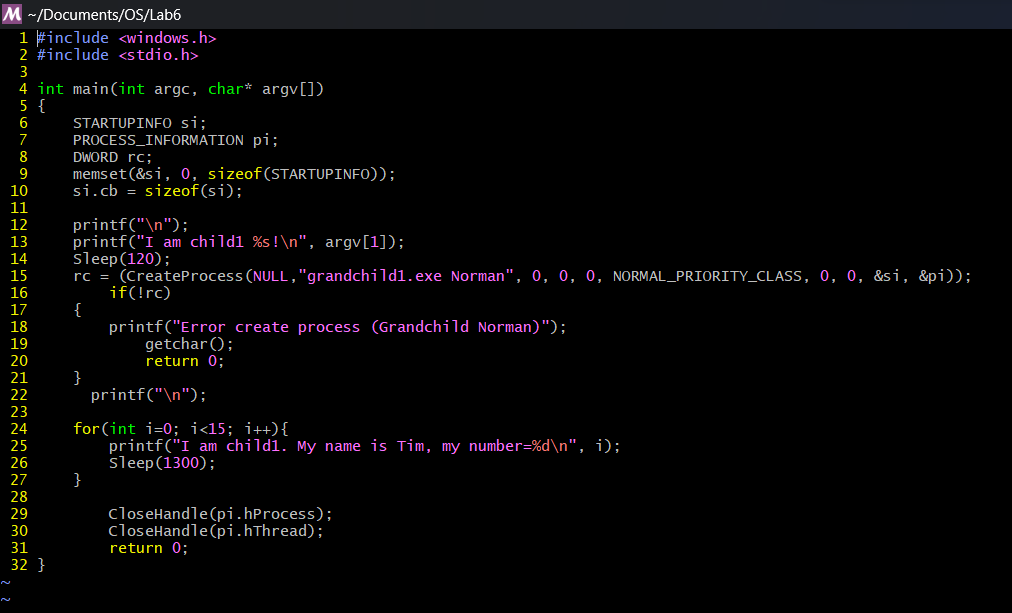
\includegraphics[width=\textwidth]{images/lab6/child1.png}
        \caption{Код программы child1.c}
    \end{figure}
    
    \begin{figure}[H]
        \centering
        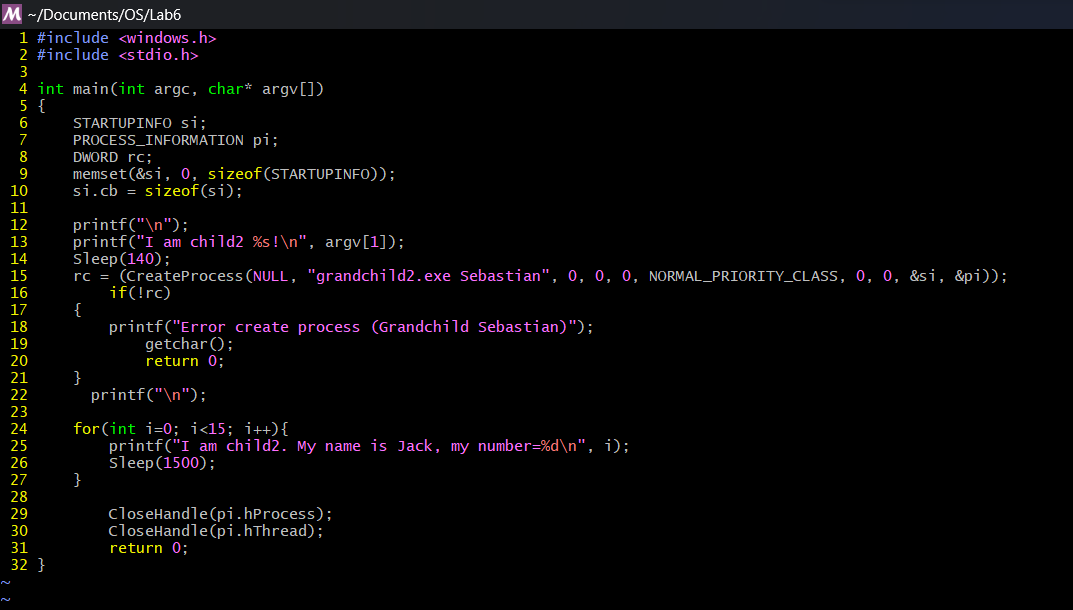
\includegraphics[width=\textwidth]{images/lab6/child2.png}
        \caption{Код программы child2.c}
    \end{figure}
    
    \begin{figure}[H]
        \centering
        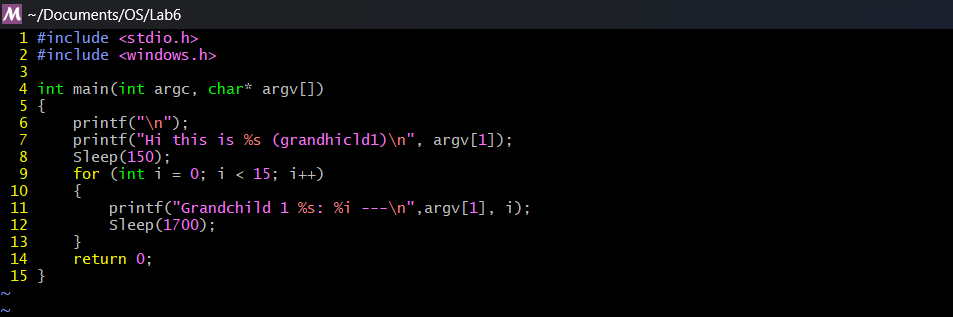
\includegraphics[width=\textwidth]{images/lab6/grandchild1.png}
        \caption{Код программы grandchild1.c}
    \end{figure}
    
    \begin{figure}[H]
        \centering
        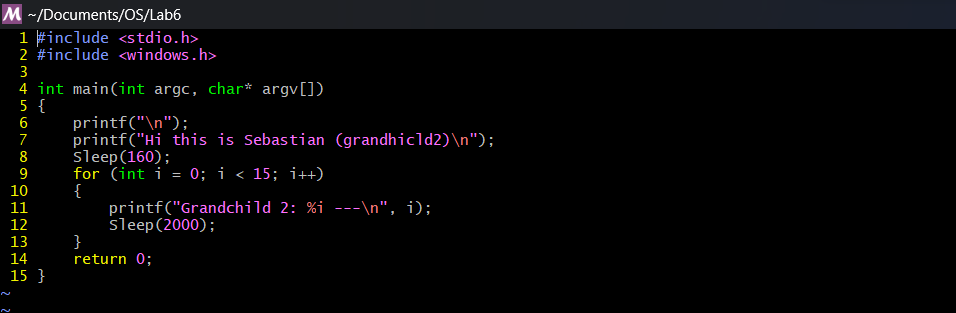
\includegraphics[width=\textwidth]{images/lab6/grandchild2.png}
        \caption{Код программы grandchild2.c}
    \end{figure}
    
    \begin{figure}[H]
        \centering
        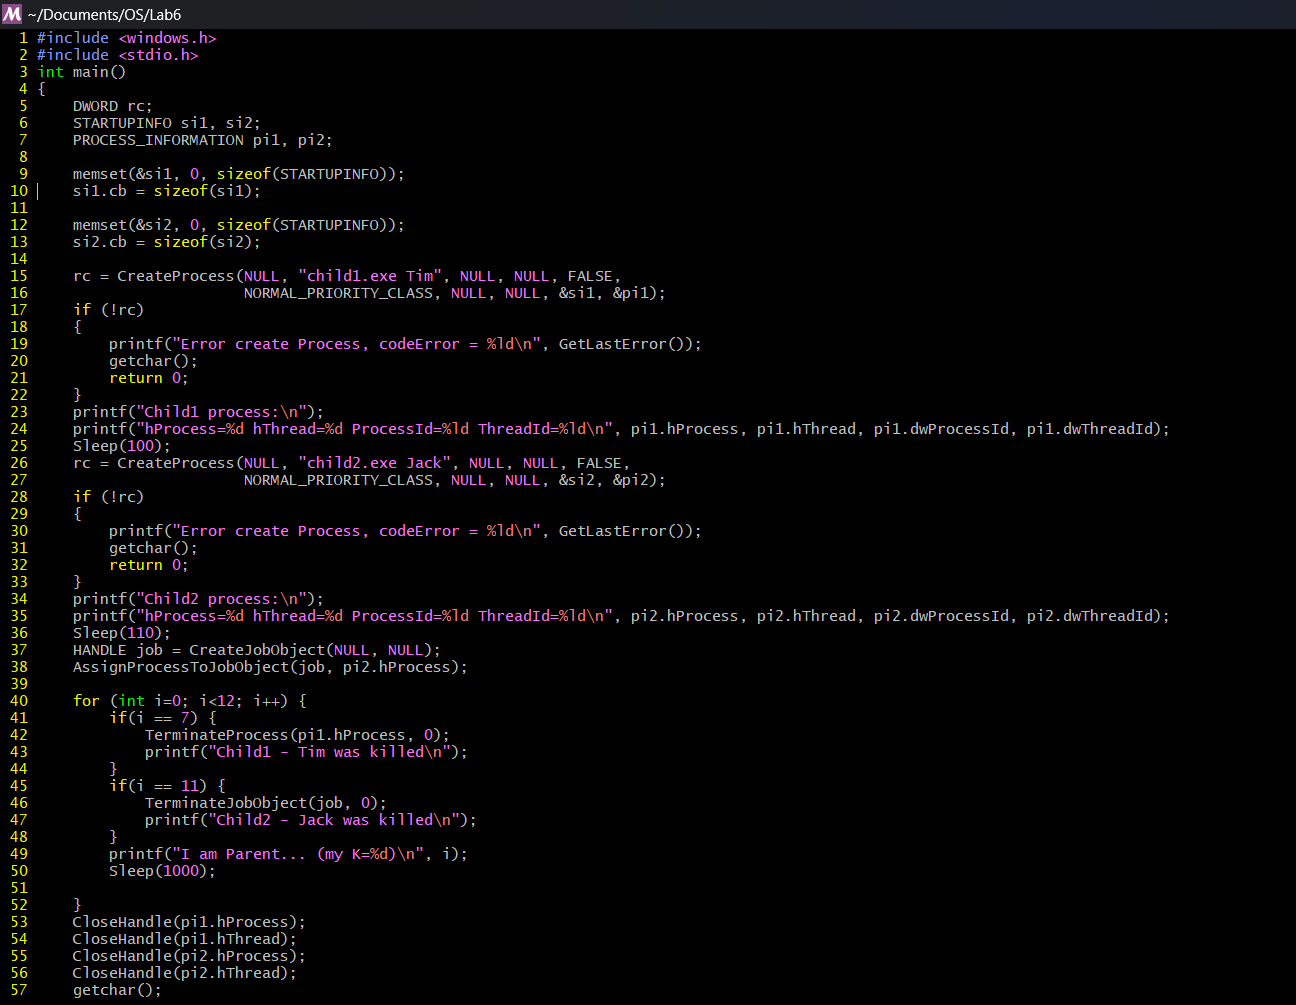
\includegraphics[width=\textwidth]{images/lab6/parent.png}
        \caption{Код программы parent.c}
    \end{figure}

    \begin{figure}[H]
        \centering
        \includegraphics[width=\textwidth]{images/lab6/result.png}
        \caption{Результат работы программ parent.c}
    \end{figure}

    \newpage

    \section*{Задание 7}

    Разработать программу с тремя дополнительными нитями (threads) относительно главной нити. Каждая из нитей должна использовать общие для всех нитей данные, представленные массивом символов, в которых записаны 20 первых букв латинского алфавита. Каждая из этих нитей на своем k-м шаге выводит со своей случайной задержкой на место «своего» столбца экрана k-ю букву из указанного массива латинских букв, причем с числом повторений, равному условному номеру нити, умноженному на два. Каждая из используемых нитей должен осуществлять вывод своим цветом, отличным от остальных нитей. На 6-м шаге главная нить делает попытку отмены первой из дополнительных нитей, а на 11-м делает попытку отмены третьей из дополнительных нитей. Первая и третья дополнительная нити в начале своей работы запрещают свою отмену. Третья нить на 13 шаге разрешает отмену, но в отложенном режиме. Точку отмены эта нить устанавливает между 16 и 17-м шагом своей работы. Все управляющие указания должны отображаться сообщениями без прокрутки экрана (в фиксированные позиции экрана).

    \subsection*{Решение}

    \begin{figure}[H]
        \centering
        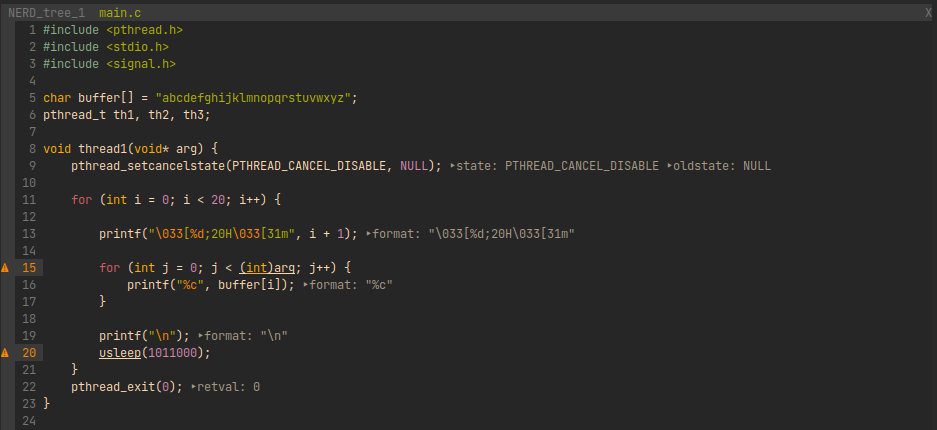
\includegraphics[width=\textwidth]{images/lab7/thread1.png}
        \caption{Код метода thread1}
    \end{figure}

    \begin{figure}[H]
        \centering
        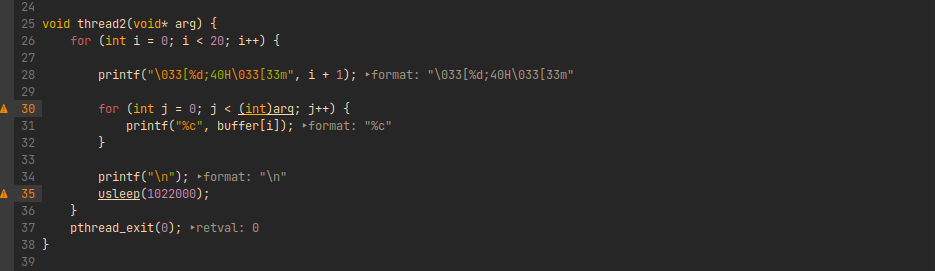
\includegraphics[width=\textwidth]{images/lab7/thread2.png}
        \caption{Код метода thread2}
    \end{figure}

    \begin{figure}[H]
        \centering
        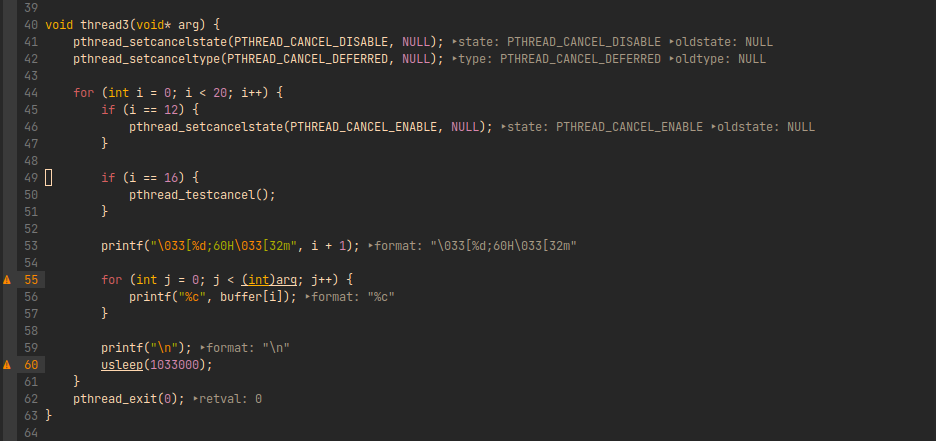
\includegraphics[width=\textwidth]{images/lab7/thread3.png}
        \caption{Код метода thread3}
    \end{figure}

    \begin{figure}[H]
        \centering
        \includegraphics[width=\textwidth]{images/lab7/main.png}
        \caption{Код метода main}
    \end{figure}

    \begin{figure}[H]
        \centering
        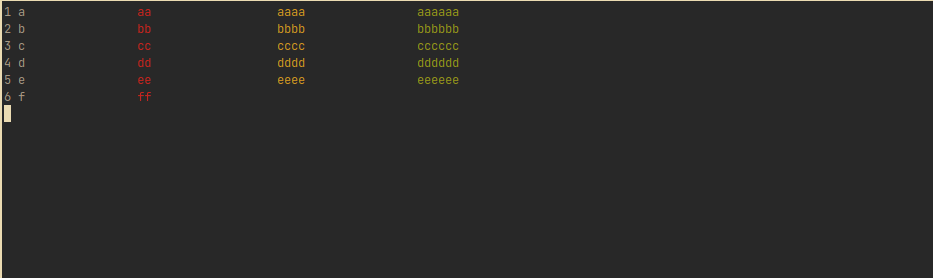
\includegraphics[width=\textwidth]{images/lab7/result1.png}
        \caption{Результат работы программы в момент работы первого потока}
    \end{figure}

    \begin{figure}[H]
        \centering
        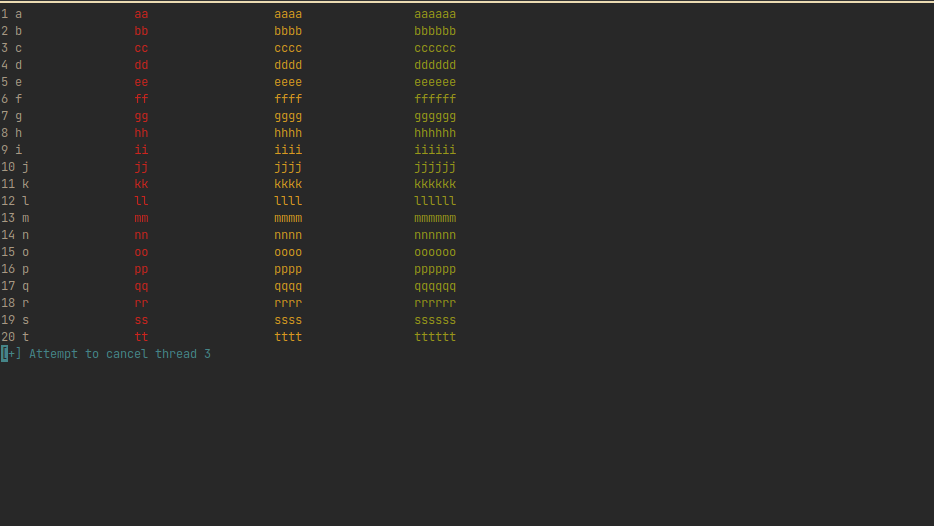
\includegraphics[width=\textwidth]{images/lab7/result2.png}
        \caption{Результат работы программы в момент работы третьего потока}
    \end{figure}

    \newpage

    \section*{Задание 8}

    Разработать многопоточную программу, отображающие на экране взаимодействие трех нитей «читателей» из общей области данных и трех «писателей», записывающих в этот буфер данные. Буфер предназначен для хранения 12 символов. Первая нить-писатель выводит латинскими буквами название города "Novosibirsk", вторая нить-писатель выводит латинскими буквами название города "Semipalatink", а третья — название города "Ekaretinburg". Такой вывод эти три нити осуществляют в два приема, первый из которых записывает половину своего текста без завершающего этот промежуточный текст нуля. Между такими половинами вывода нити производят задержку на случайную величину миллисекунд, но не более 1 сек. После вывода своего текста в буфер каждая нить-писатель переходит в ожидание порядка 2-3 сек до следующей попытки записи в буфер. Нити-читатели - через случайный интервал порядка 300 мсек - читают данные из буфера, если это позволяют средства синхронизации доступа между нитями, и вывод прочитанный текст на экран, каждая в свой столбец. Каждый вывод нити-читателя осуществляется в новую строку своего столбца, поэтому суммарные действия вывода в таких нитях предусмотреть только для 20 - 24 строк. Синхронизацию осуществить с помощью семафоров.

    \begin{figure}[H]
        \centering
        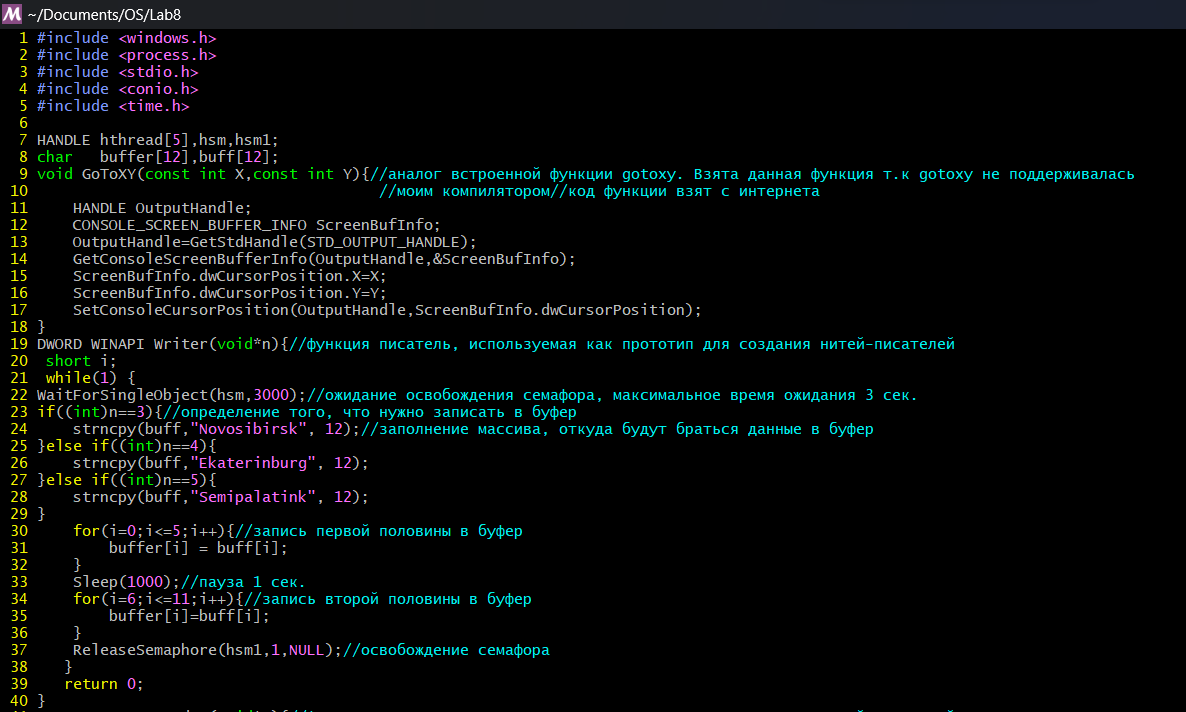
\includegraphics[width=\textwidth]{images/lab8/main1.png}
        \caption{Код программы main1.c}
    \end{figure}

    \begin{figure}[H]
        \centering
        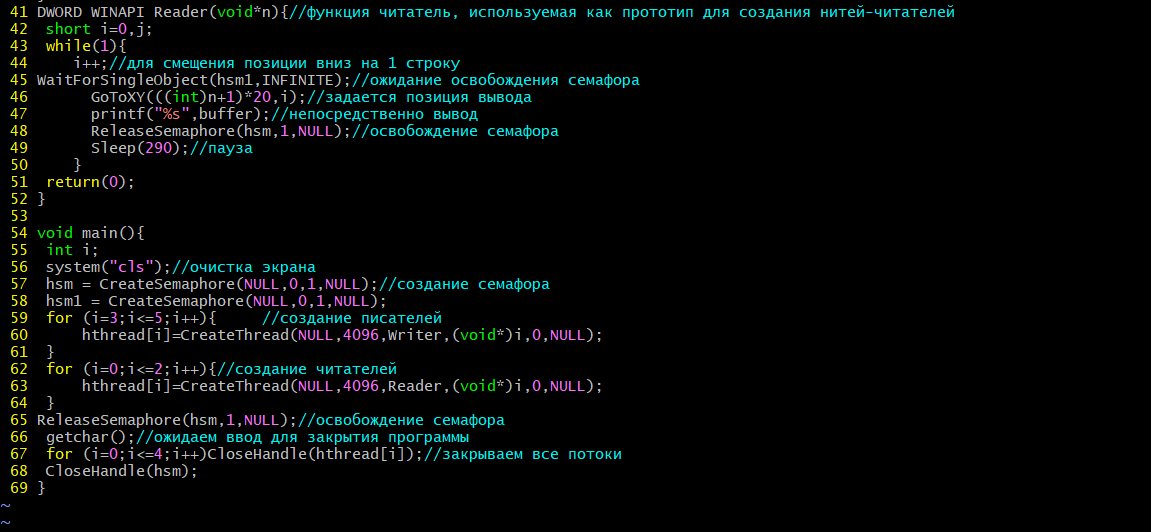
\includegraphics[width=\textwidth]{images/lab8/main2.png}
        \caption{Код программы main2.c}
    \end{figure}

    \begin{figure}[H]
        \centering
        \includegraphics[width=\textwidth]{images/lab8/result.png}
        \caption{Результат работы программ main.c}
    \end{figure}

    \newpage

    \section*{Задание 9}

    Разработать программы в ОС Windows для двух отдельных процессов, использующих общую память. В первой программе должна создаваться разделяемая память и семафор для взаимодействия между процессами. Во второй открывается доступ к этой же разделяемой памяти и семафору. Первая программа должна после задержки в 10 - 15 секунд записать какой-то текст в разделяемую память и указать его готовность с помощью семафора, а вторая программа должна вначале прочитать текстовую информацию из того места разделяемой памяти, где она должна появиться и выдать полученную информацию на экран с примечанием о существе действия, затем перейти к ожиданию разрешающего значения семафора и только после его завершения выдать на экран содержимое из разделяемой памяти с соответствующим примечанием. Вместо семафора в Windows можно использовать событие или мьютекс. Обе программы должны после получения действующего указателя на область общей памяти вывести адрес этой области в консольное окно с соответствующими пояснениями.

    Первая программа, кроме того, после формирования данных для второго процесса, должна запросить 1000 байтов дополнительной памяти с помощью универсальной функции VirtualAlloc и записать в эту область памяти, начиная с ее начала, сколько возможно символов латинского алфавита, записывая эти символы, пропуская по 399 свободных байтов (т.е. записывая 'a' в байт с нулевым смещением этой области памяти, затем 'b' в байт со смещением 400, далее 'c' в байт со смещением 800 и т.д., выполняя такое продвижение на 400 байтов по крайнем мере 15 раз). Каждую такую запись байта сопровождать детальным сообщением о действии и числовым значением адреса, по которому размещается этот байт в памяти. Наблюдаемые результаты объяснить.

    \begin{figure}[H]
        \centering
        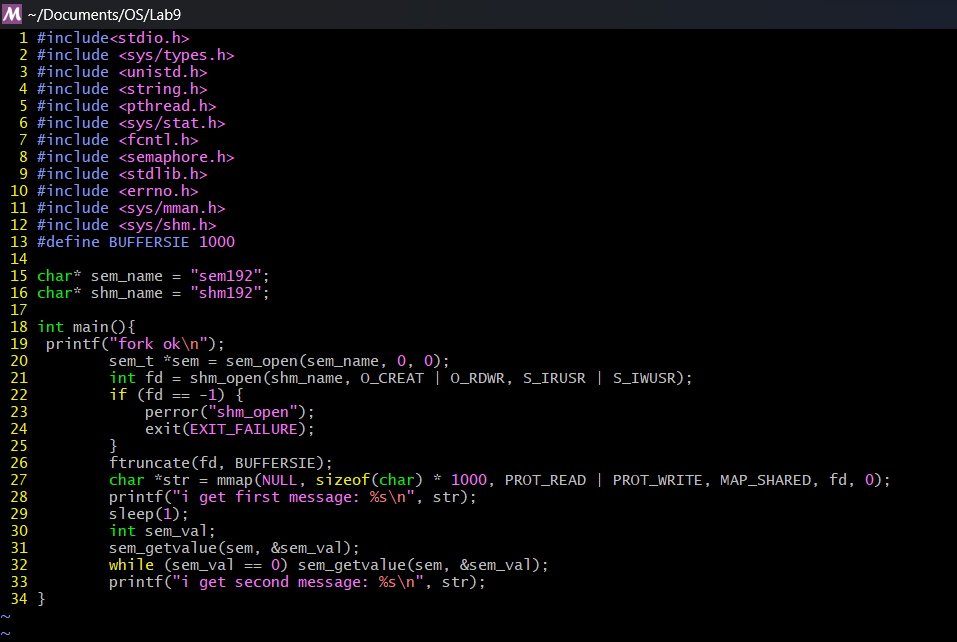
\includegraphics[width=\textwidth]{images/lab9/app.png}
        \caption{Код программы app.c}
    \end{figure}

    \begin{figure}[H]
        \centering
        \includegraphics[width=\textwidth]{images/lab9/main.png}
        \caption{Код программы main.c}
    \end{figure}

    \begin{figure}[H]
        \centering
        \includegraphics[width=\textwidth]{images/lab9/result.png}
        \caption{Результат работы программ app.c и main.c}
    \end{figure}

    \newpage
    
\end{document}
